\section{Viga estática continua B4, B8, B15 y B16}
\label{sec:viga-b16}
 
\subsection{Geometría y ubicación}
 
La viga B4, B8, B15 y B16 son vigas continuas de cuatro tramos ubicadas en el subterráneo. Su análisis se realiza mediante modelación en SAP2000, obteniendo la envolvente de esfuerzos para las combinaciones de carga gravitacional. La geometría de cada tramo se resume en la Tabla~\ref{tab:viga-tramos}.
 
\begin{table}[h!]
\centering
\caption{Longitudes y condiciones de borde de la viga continua.}
\label{tab:viga-tramos}
\begin{tabular}{lcc}
\toprule
Tramo & Longitud (m) & Condición de borde \\
\midrule
$L_1$ & 5{,}49 & Un extremo continuo \\
$L_2$ & 5{,}95 & Ambos extremos continuos \\
$L_3$ & 6{,}41 & Ambos extremos continuos \\
$L_4$ & 8{,}35 & Un extremo continuo \\
\bottomrule
\end{tabular}
\end{table}
 
\noindent Las propiedades de la sección transversal y los materiales empleados son:
 
\begin{itemize}
    \item Sección: $b = 25$ cm, $h = 50$ cm; recubrimiento $r = 5$ cm; altura útil $d = 45$ cm
    \item Hormigón G35 según NCh170: $f'_c = 350\ \text{kg/cm}^2\ (35\ \text{MPa})$; $E_c = 27{,}81\ \text{GPa}$
    \item Acero A630-420H según NCh204: $f_y = 4200\ \text{kg/cm}^2\ (420\ \text{MPa})$; $E_s = 200\ \text{GPa}$
    \item $A_g = 0{,}125\ \text{m}^2$; $I_g = 2{,}604 \times 10^{-3}\ \text{m}^4$
\end{itemize}
 
La altura mínima según ACI~318-19 se verifica en los cuatro tramos.
 
\subsection{Cargas tributarias}
 
Las cargas distribuidas sobre la viga se determinan mediante el método de los 45°, considerando el peso propio del hormigón ($\gamma = 2500\ \text{kgf/m}^3$), la carga muerta adicional de losa ($PP = 100\ \text{kgf/m}^2$) y la sobrecarga de uso ($SC = 500\ \text{kgf/m}^2$). Los valores por tramo se presentan en la Tabla~\ref{tab:viga-cargas}.
 
\begin{table}[h!]
\centering
\caption{Cargas distribuidas por tramo de la viga continua.}
\label{tab:viga-cargas}
\begin{tabular}{lcc}
\toprule
Tramo & $w_{PP}$ (tonf/m) & $w_{SC}$ (tonf/m) \\
\midrule
$L_1$ & 1{,}657 & 1{,}744 \\
$L_2$ & 1{,}750 & 1{,}843 \\
$L_3$ & 1{,}830 & 1{,}927 \\
$L_4$ & 2{,}016 & 2{,}123 \\
\bottomrule
\end{tabular}
\end{table}
 
La combinación de carga última se aplica conforme a ACI~318-19:
 
\begin{equation}
    q_u = 1{,}2\,PP + 1{,}6\,SC
\end{equation}
 
\subsection{Esfuerzos de diseño}
 
Los esfuerzos de diseño se obtienen del modelo en SAP2000. La sección crítica corresponde al apoyo con mayor momento negativo, que gobierna el diseño a flexión. Los valores determinantes son:
 
\begin{align}
    M_{u,\max} &= +18{,}13\ \text{tonf}{\cdot}\text{m} \\
    M_{u,\min} &= -24{,}26\ \text{tonf}{\cdot}\text{m} \quad \text{(sección crítica)} \\
    V_{u,\max} &= +9{,}58\ \text{tonf} \\
    V_{u,\min} &= -17{,}61\ \text{tonf} \quad \text{(corte de diseño)}
\end{align}
 
\subsection{Diseño a flexión}
 
\subsubsection{Armadura mínima y máxima}
 
Las cuantías límite se determinan conforme a ACI~318-19:
 
\begin{equation}
    A_{s,\min} = \max\!\left(\frac{0{,}25\sqrt{f'_c}}{f_y}\,b\,d\ ;\ \frac{1{,}4}{f_y}\,b\,d\right) = 3{,}75\ \text{cm}^2
\end{equation}
 
\begin{equation}
    A_{s,\max} = 23{,}91\ \text{cm}^2 \quad (\rho_{\max} = 0{,}02125)
\end{equation}
 
\subsubsection{Armadura adoptada y verificaciones}
 
Se adoptan $4\,\phi 25$, que aportan $A_s = 19{,}63\ \text{cm}^2$, valor dentro del rango admisible. Con esta armadura se verifican la profundidad del bloque de compresiones, la deformación unitaria del acero en tracción y la resistencia a flexión:
 
\begin{align}
    a &= \frac{A_s\,f_y}{0{,}85\,f'_c\,b} = 0{,}1109\ \text{m} \\
    c &= \frac{a}{\beta_1} = \frac{0{,}1109}{0{,}80} = 0{,}1386\ \text{m} \\
    \varepsilon_s &= 0{,}003\cdot\frac{d - c}{c} = 0{,}00674 > 0{,}005
\end{align}
 
La deformación unitaria del acero supera 0{,}005, por lo que la sección está \textbf{controlada por tracción} y el factor de reducción es $\phi = 0{,}90$. La resistencia nominal y de diseño resultan:
 
\begin{align}
    M_n &= 325{,}38\ \text{kN}{\cdot}\text{m} \\
    \phi M_n &= 292{,}84\ \text{kN}{\cdot}\text{m}\ \geq\ M_u = 238{,}03\ \text{kN}{\cdot}\text{m} \quad Cumple
\end{align}
 
\subsection{Diseño a corte}
 
La resistencia al corte del hormigón se calcula conforme a ACI~318-19:
 
\begin{align}
    V_u &= 172{,}75\ \text{kN} \\
    V_c &= 0{,}17\sqrt{f'_c}\,b\,d = 113{,}15\ \text{kN} \\
    \tfrac{1}{2}\,\phi\,V_c &= 42{,}43\ \text{kN} < V_u \quad \Rightarrow\ \text{se requiere armadura de corte}
\end{align}
 
El aporte requerido de la armadura transversal es:
 
\begin{equation}
    V_s = \frac{V_u}{\phi} - V_c = 117{,}19\ \text{kN}
\end{equation}
 
Dado que $V_s < 0{,}33\sqrt{f'_c}\,b\,d = 219{,}63\ \text{kN}$, el espaciamiento máximo es $s_{\max} = d/2 = 0{,}225\ \text{m}$. Se adoptan estribos $\phi 10$ @ $225\ \text{mm}$, con lo que:
 
\begin{align}
    A_{v} &= 157{,}08\ \text{mm}^2\ >\ A_{v,\min} = 49{,}12\ \text{mm}^2 \quad Cumple \\
    \phi V_n &= 183{,}82\ \text{kN}\ \geq\ V_u = 172{,}75\ \text{kN} \quad Cumple
\end{align}
 
\subsection{Resumen del diseño}
 
La Tabla~\ref{tab:viga-resumen} muestra los resultados del diseño de la viga continua.
 
\begin{table}[h!]
\centering
\caption{Resumen del diseño de la viga estática continua.}
\label{tab:viga-resumen}
\begin{tabular}{ll}
\toprule
Parámetro & Valor \\
\midrule
Sección & $25 \times 50$ cm \\
Armadura longitudinal & $4\,\phi 25$ \\
Armadura transversal & $\phi 10$ @ 225 mm \\
$\phi M_n / M_u$ & 1{,}23 \\
$\phi V_n / V_u$ & 1{,}06 \\
$\varepsilon_s$ & 0{,}00674 (controlado por tracción) \\
\bottomrule
\end{tabular}
\end{table}

\subsection{Esquema de sección transversal mas desfavorable L4}

La Figura~\ref{fig:seccionB16} muestra el corte de la sección más desfavorable de la viga B16,
correspondiente al apoyo interior de mayor momento negativo. Se indican la armadura longitudinal
de flexión (4$\phi$25), los estribos de corte ($\phi$10@225\,mm) y las dimensiones de la sección diseñada.

\begin{figure}[H]
    \centering
    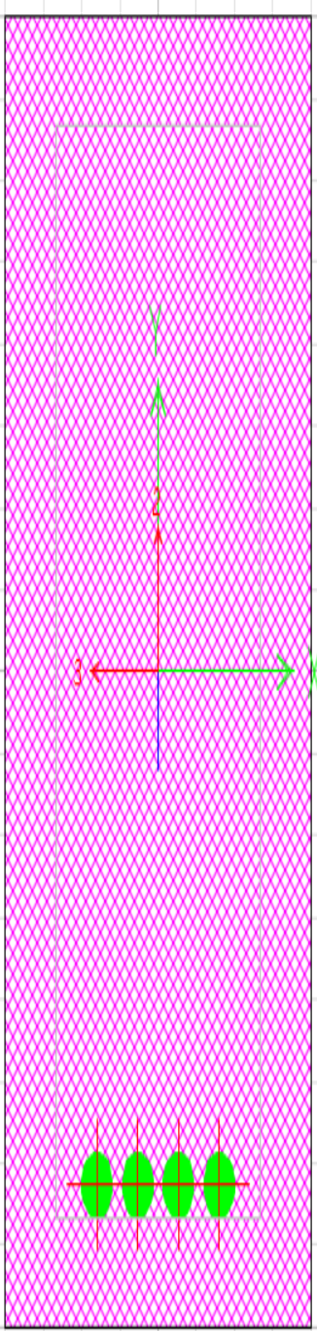
\includegraphics[width=0.15\textwidth]{Secciones/imagenes/L4}
    \caption{Corte de sección transversal de la viga B16 en la sección más desfavorable.}
    \label{fig:seccionB16}
\end{figure}
  
\subsection{Diagramas de esfuerzos}
 
Los diagramas de momento flector y fuerza de corte se obtienen de la envolvente del modelo en SAP2000 bajo la combinación de carga última $q_u = 1{,}2\,PP + 1{,}6\,SC$. Se presentan en las Figuras~\ref{fig:momento-viga} y~\ref{fig:corte-viga}.
 
\begin{figure}[H]
    \centering
    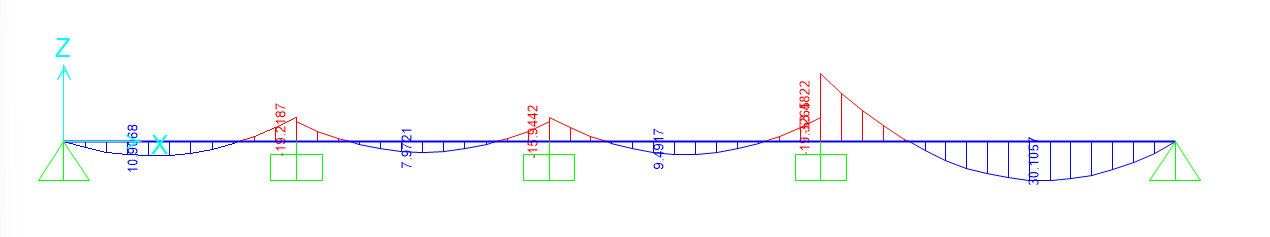
\includegraphics[width=0.9\textwidth]{Secciones/imagenes/momentViga.png}
    \caption{Diagrama de momento flector $M_u$ en la viga continua (tonf$\cdot$m).}
    \label{fig:momento-viga}
\end{figure}
 
\begin{figure}[H]
    \centering
    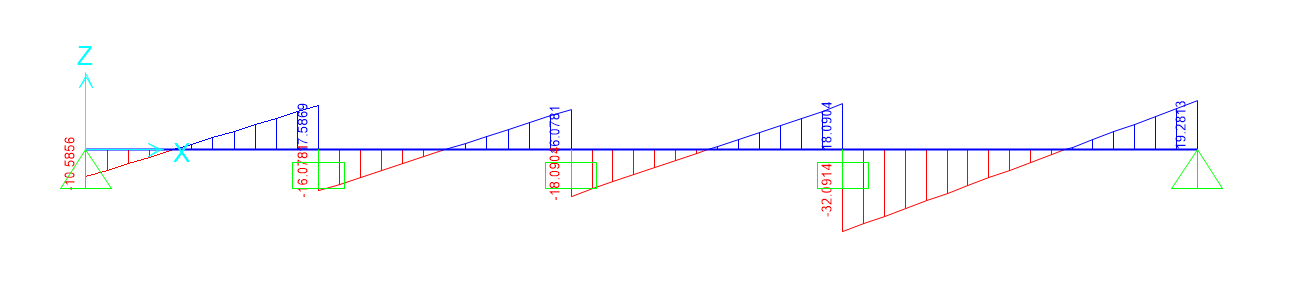
\includegraphics[width=0.9\textwidth]{Secciones/imagenes/shearViga.png}
    \caption{Diagrama de fuerza de corte $V_u$ en la viga continua (tonf).}
    \label{fig:corte-viga}
\end{figure}
 
\subsection{Deformación y verificación de flechas}
 
\subsubsection{Momento de inercia efectivo}
 
Dado que la viga se encuentra fisurada bajo carga de servicio, se requiere previamente la inercia fisurada $I_{cr}$ y el momento de fisuración $M_{cr}$.
 
La razón modular resulta $n = E_s/E_c = 200{.}000/27{.}806 = 7{,}19$. Con tres barras $\phi 18$ ($A_s = 763{,}4\ \text{mm}^2$), la posición del eje neutro fisurado se obtiene de la ecuación cuadrática:
 
\begin{equation}
    \frac{b}{2}\,c^2 + n\,A_s\,c - n\,A_s\,d = 0 \quad \Rightarrow \quad c = 12{,}03\ \text{cm}
\end{equation}
 
La inercia fisurada y el momento de fisuración son:
 
\begin{align}
    I_{cr} &= \frac{b\,c^3}{3} + n\,A_s\,(d-c)^2 = 7{,}420 \times 10^{-4}\ \text{m}^4 \\
    f_r &= 0{,}62\,\lambda\sqrt{f'_c} = 3{,}668\ \text{MPa} \\
    M_{cr} &= \frac{f_r\,I_g}{y_t} = 3{,}90\ \text{tonf}{\cdot}\text{m}
\end{align}
 
El momento de servicio $M_a = 7{,}11\ \text{tonf}{\cdot}\text{m}$ supera $(2/3)\,M_{cr} = 2{,}60\ \text{tonf}{\cdot}\text{m}$, confirmando que la sección está fisurada. La inercia efectiva resulta:
 
\begin{equation}
    I_e = \frac{I_{cr}}{1 - \eta\left(\dfrac{M_{cr}}{M_a}\right)^2} = 9{,}447 \times 10^{-4}\ \text{m}^4 \qquad \left(I_{cr} \leq I_e \leq I_g\ \right)
\end{equation}
 
donde $\eta = 1 - I_{cr}/I_g = 0{,}715$.
 
\subsubsection{Flecha instantánea}
 
La flecha elástica instantánea se estima mediante:
 
\begin{equation}
    f_i = \frac{M_a\,L^2}{\alpha\,E_c\,I_e}
\end{equation}
 
Se evalúan dos condiciones de apoyo que acoten el resultado real de la viga continua: apoyo simple--apoyo simple ($\alpha = 9{,}6$) y empotrado--apoyo simple ($\alpha = 16{,}0$). Los resultados se presentan en la Tabla~\ref{tab:flechas}.
 
\subsubsection{Flecha diferida por fluencia lenta}
 
La deformación adicional a largo plazo se estima con la expresión simplificada de ACI~318-19:
 
\begin{equation}
    \Delta_{\text{creep}} = \lambda_\Delta \cdot f_i \qquad \text{con} \qquad \lambda_\Delta = \frac{\xi}{1 + 50\,\rho'}
\end{equation}
 
Sin armadura de compresión ($\rho' = 0$) y para un período de carga de 5 años o más ($\xi = 2{,}0$), se obtiene $\lambda_\Delta = 2{,}0$. La flecha total resulta:
 
\begin{equation}
    \Delta_{\text{total}} = (1 + \lambda_\Delta)\,f_i = 3{,}0\,f_i
\end{equation}
 
\subsubsection{Verificación de deflexiones admisibles}
 
La verificación se realiza según ACI~318-19, tabla 24.2.2. Considerando que el 100\,\% de la carga es permanente, la sobrecarga variable es nula ($\Delta_{CV} = 0$), por lo que el caso crítico es el Caso~4 ($\Delta_{\text{creep}} + \Delta_{CV}$) con límite $\ell/240$.
 
\begin{table}[H]
\centering
\small
\caption{Flechas instantánea, diferida y total por condición de apoyo.}
\label{tab:flechas}
\begin{tabular}{lcccccc}
\toprule
Condición de apoyo & $\alpha$ & $f_i$ (mm) & $\Delta_{\text{creep}}$ (mm) & $\Delta_{\text{total}}$ (mm) & Límite $\ell/240$ (mm) & Verif. \\
\midrule
Apoyo simple -- apoyo simple   & 9{,}6  & 8{,}34 & 16{,}67 & 25{,}01 & 22{,}88 & \checkmark \\
Empotrado -- apoyo simple      & 16{,}0 & 5{,}00 & 10{,}00 & 15{,}01 & 22{,}88 & \checkmark \\
\bottomrule
\end{tabular}
\end{table}

Ambas condiciones cumplen el límite $\ell/240$ del Caso~4. La condición de apoyo simple--apoyo simple representa la situación más desfavorable con $\Delta_{\text{creep}} = 16{,}67\ \text{mm} \leq 22{,}88\ \text{mm}$, mientras que la condición empotrado--apoyo simple, más representativa de la viga continua, cumple holgadamente con $\Delta_{\text{creep}} = 10{,}00\ \text{mm} \leq 22{,}88\ \text{mm}$. En consecuencia, la deformación de la viga continua se considera aceptable.
